\usetikzlibrary{patterns}
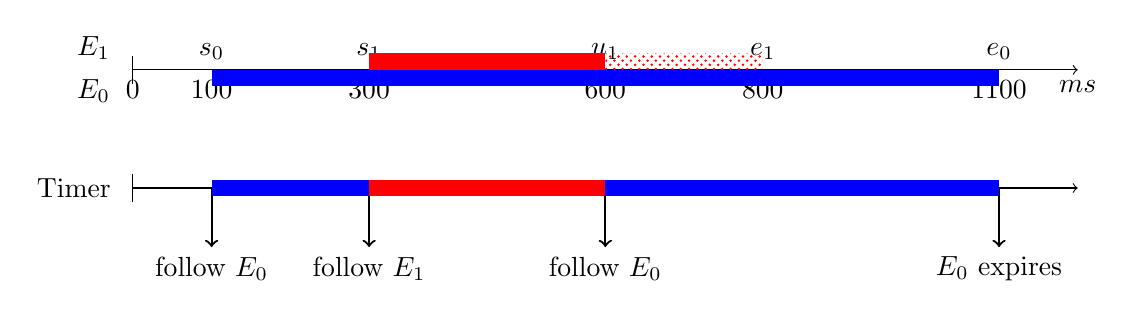
\begin{tikzpicture}[]
	% draw horizontal line
	\draw (0.25,0) node {Timer};
	\draw[->] (1,0) -- ++(12,0);

	%\draw (0,1) node {errors};
	\draw[->] (1,1.5) -- ++(12,0);

	% draw vertical lines
	%\foreach \x in {1,2,4,7,11}
	%  \draw (\x cm,1cm+3pt) -- (\x cm,1cm-3pt);

	\draw (1,1.5cm+5pt) -- (1,1.5cm-5pt);
	\draw (1,5pt) -- (1,-5pt);

	% draw nodes
	\draw (0.5,1.5) node[below=.05] {$E_0$} node[above=.05] {$E_1$};
	\draw (1,1.5) node[below=.5] {$0$};
	\draw (2,1.5) node[below=.5] {$100$} node[above=.25] {$s_0$};
	\draw (4,1.5) node[below=.5] {$300$} node[above=.25] {$s_1$};
	\draw (7,1.5) node[below=.5] {$600$} node[above=.25] {$u_1$};
	\draw (9,1.5) node[below=.5] {$800$} node[above=.25] {$e_1$};
	\draw (12,1.5) node[below=.5] {$1100$} node[above=.25] {$e_0$};
	\draw (13,1.5) node[below=.5] {$ms$};

	%\draw (2,0) node[below=.25] {Track $e_0$};
	%\draw (4,0) node[below=.25] {Track $e_1$};
	%\draw (7,0) node[below=.25] {Track $e_0$};
	%\draw (11,0) node[below=.25] {Timeout $e_0$};

	\fill[blue] (2,1.5) rectangle ++(10,-6pt);
	\fill[red] (4,1.5) rectangle ++(3,6pt);
	\fill[red, pattern=crosshatch dots, pattern color=red] (7,1.5) rectangle ++(2,6pt);

	\draw [thick,->] (2,0) -- ++(0,-.75);
	\node[align=center, anchor=north] at (2,-.75) {follow $E_0$};

	\draw [thick,->] (4,0) -- ++(0,-.75);
	\node[align=center, anchor=north] at (4,-.75) {follow $E_1$};

	\draw [thick,->] (7,0) -- ++(0,-.75);
	\node[align=center, anchor=north] at (7,-.75) {follow $E_0$};

	\draw [thick,->] (12,0) -- ++(0,-.75);
	\node[align=center, anchor=north] at (12,-.75) {$E_0$ expires};

	\fill[blue] (2,-3pt) rectangle (4,3pt);
	\fill[red] (4,-3pt) rectangle (7,3pt);
	\fill[blue] (7,-3pt) rectangle (12,3pt);
\end{tikzpicture}